\chapter{Experiments}
\label{chap:exp}
This chapter describes all experiments and their results. The first part is dedicated to presentation of different experiement hyperparameters, that are in many cases common to all tasks, followed by the description of each task and a discussion of results.
\section{A description of training hyperparameters}
\label{sec:expe}
\subsection{General experiment setup (EXPE)}
Training is performed in one of the following settings:
\begin{itemize}
\item \textbf{base}: Baseline implementation (described separately for each task, typically without using advanced language models).
\item \textbf{ls}: This setup uses same setting as baseline implementation but with label smoothing.
\item \textbf{embed}: BERT-like language model is used only to generate static embeddings in advance. Non-BERT part of the model is trained with BERT layers frozen (pre-trained, not changed during training).
\item \textbf{full}: This options means training the whole model from the beginning (in contrast to \textit{fine} option), but the classification head is not simplified (in contrast to \textit{simple} option).
\item \textbf{fine}: Fine-tuning consist of dividing the training time into two parts. First part of training is same to \textit{embed} setting. In the second part, the whole model is trained together (as in \textit{full}).
\item \textbf{simple}: Model architecture is reduced to BERT layers with a simple classification head. This is a basic setting for all sentiment analysis experiments.\footnote{For tagging and lemmatization, all previously mentioned EXPE setups are performed with more sophisticated classification head than in \textit{simple} version.} 
\end{itemize}
\subsection{Training data}
Tagging and lemmatization tasks use the same set of data for all experiments, so there is no need for separate description. Sentiment analysis task, however, uses three possible options as a selection of training data:
\begin{itemize}
\item \textbf{mall|facebook|csfd}: Model is trained and evaluated on the (sub)set of Czech datasets.
\item \textbf{zero}: Model is trained on English sentiment analysis dataset, but evaluated on Czech data.
\item \textbf{eng}: Model is trained on the combination of Czech and English training data (and evaluated again on the Czech data). %TODO pridat jeste jednotlive ceske datasety
\end{itemize}
\subsection{Learning rate scheduling type (LRTYPE)}
Most experiments are expected to perform better with some kind of learning rate scheduling. This work implements three types of learning rate scheduling:
\begin{itemize}
\item \textbf{simple} \textit{Simple} option indicates no more complex learning rate scheduling than setting different learning rates for different epochs in advance.
\item \textbf{isrd} %TODO citovat 
\textit{isrd} means inverse square root learning rate decay defined by formula: $$1/\sqrt{n},$$  where $n$ is the current iteration.
\item \textbf{cos}: Another learning rate scheduling used in this work is \textit{cosine decay}, %TODO citovat
which applies the following formula: $$lr=lr_{min}^{i} + \frac{1}{2}\bigg(lr_{max}^{i} - lr_{min}^{i}\bigg)\bigg(1+\cos\bigg(\frac{T_{curr}}{T_i}\pi\bigg)\bigg),$$ where $lr_{min}^{i}$ is the range of the learning rate, $T_{curr}$ is the current epoch number, and $T_i$ is the number of epochs after which the learning rate is restarted, i.e. increased to the $lr_{max}^{i}$ value and $T_curr$ is reset to 0.
\end{itemize}
Both \textit{cos} and \textit{isrd} are combined with \textit{warmup}. Learning rate is linearly increasing for first $k$ steps (one epoch in all experiments) from zero to the value in hyperparameters and than starts the decay.

\subsection{Model layers selected for embeddings (LAYERS)}
As discussed in the previous chapter, it is unclear how to extract best embeddings from the language model, especially which layers to take into account. According to the results published in \citep{Devlin2018} and \citep(Kondratyuk2019), we consider the following two promising approaches:
\begin{itemize}
\item \textbf{four}: Last four layers of the model are averaged to obtain final embeddings.
\item \textbf{att}: Layer attention performs weighted sum of all model layers, and the weights are trained during training together with the rest of the model.
\end{itemize}
Experiments are also performed with different learning rates (LR), batch size (BATCH), and a number of epochs (EPOCH). 
Technical details needed for running scripts with the right arguments can be found in chapter \ref{chap:impl}.

\subsection{Metrics}
Metrics used for evaluation in this work are \textit{accuracy} and \textit{F1 score}. 
Accuracy is a percentage of correctly classified samples out of all samples, and it is the basic metric for all classification tasks (not only in this thesis). Accuracy can be sometimes misleading \citep{davisoriginal}, and there exist other metrics that can better reflect experimenter's goals. One of them is F1 score, which is used together with accuracy for evaluation of sentiment analysis task due to comparability of results. F1 score is defined in terms of precision and recall. Precision  
$$\mathit{precision} = \frac{TP}{TP + FP}$$\footnote{TP stands for true positive = number of samples correctly labelled as 1, FP (=false positives) are incorrectly labelled as 1, FN (=false negatives) is defined similarly.} express credibility of a positive result, e.g., if positive result means  a need of surgery, it is definitely unwanted to have low precision and perform many dangerous and expensive surgeries unnecessarily. Recall, defined as: $$\mathit{recall} = \frac{TP}{TP + FN},$$,
on the other hand tells us how many positives are captured. For example: \textit{How likely I am to be pregnant with a negative pregnancy test?} F1 score formula for binary classification is than defined as
$$F1 = 2 \cdot \frac{precision \cdot recall}{precision + recall}.$$
For multi-class classification, precision and recall needs to be redefined. F1 score can be computed per-class (for every class, binary classification of being in the class is taken). Per-class scores can be combined in one of following ways:
\begin{itemize}
\item macro-F1: average of per-class scores,
\item weighted-F1: average as before, but weighted by the number of samples in each class,
\item micro-F1: equals to accuracy.
\end{itemize}
\par
\newpage
\section{Lemmatization and part-of-speech tagging}
\label{chap:tag}
Lemmatization and \acrshort{pos} tagging tasks are categorized as morphological analysis, share the same architecture and trained network and they will be described together in this section.
\subsection{Task Definition}

\paragraph{\textbf{POS tagging}} \mbox{}\\
\textit{input}: a sequence of  words \\
\textit{output}: tag (for each word), which contains not only part-of-speech (e.g. noun, pronoun, punctuation mark) but also other morphological analysis (case, tense, etc) corresponding to 15-places morphological tagging system by \cite{Hajic2004}. Description of each position can be found in table \ref{Tab:tagset}.

\paragraph{\textbf{Lemmatization}} \mbox{}\\
\textit{input:} a sequence of words \\
\textit{output:} lemma (for each word) -- a base form of a given words, for example nominative of singular for nouns or infinitive for verbs. In this work, lemmatization is treated as a classification problem with classes coresponding to generating rules which transform an input word into target lemma. For example of such rules see figure \ref{fig:lemma_rules}. \\

\begin{table}[!ht]
\centering
\begin{tabular}{ |c|c|c| } 
 \hline
 Position & Name & Description \\ 
 \hline \hline
 1 & POS & Part of speech \\ \hline
 2 & SubPOS & Detailed part of speech \\ \hline
  3 & Gender & Gender \\ \hline
4 & Number & Number \\\hline
  5 & Case & Case \\ \hline
 6 & PossGender & Possessor's gender \\\hline
  7 & PossNumber & Possessor's number \\ \hline
8 & Person & Person \\\hline
  9 & Tense & Tense \\ \hline
 10 & Grade & Degree of comparison\\\hline
  11 & Negation & Negation \\ \hline
 12 & Voice & Voice \\\hline
 13 & Reserve1 & Reserve \\ \hline
14 & Reserve2 & Reserve \\\hline
  15 & Var & Variant, style \\ 
 \hline
\end{tabular}
\caption[Czech morphological tags]{Czech morphology developement is dated from 1989 \citep{Hajic2004} 
and in description of words uses 15-places morphological tags as described in this table taken from \url{https://ufal.mff.cuni.cz/pdt2.0/doc/manuals/en/m-layer/html/ch02s02s01.html}. For more detailed  description or for exploration of predictions given by this work is recommended to use website of Institute of Theoretical and Computational linguistics: \url{http://utkl.ff.cuni.cz/~skoumal/morfo/?pos=11\&val=1}, although they use slightly different set with additional 16 position. }
\label{Tab:tagset}
\end{table}

\paragraph{Metrics} Accuracy is used for the evaluation and is reported separately for several options -- only tags/lemmas, accuracy of joint classification of tags and lemmas, and  also all three variants with an usage of a morphological dictionary (this option is described in more detail in \ref{sub:dataset}).

\begin{figure}[!ht]
\centering
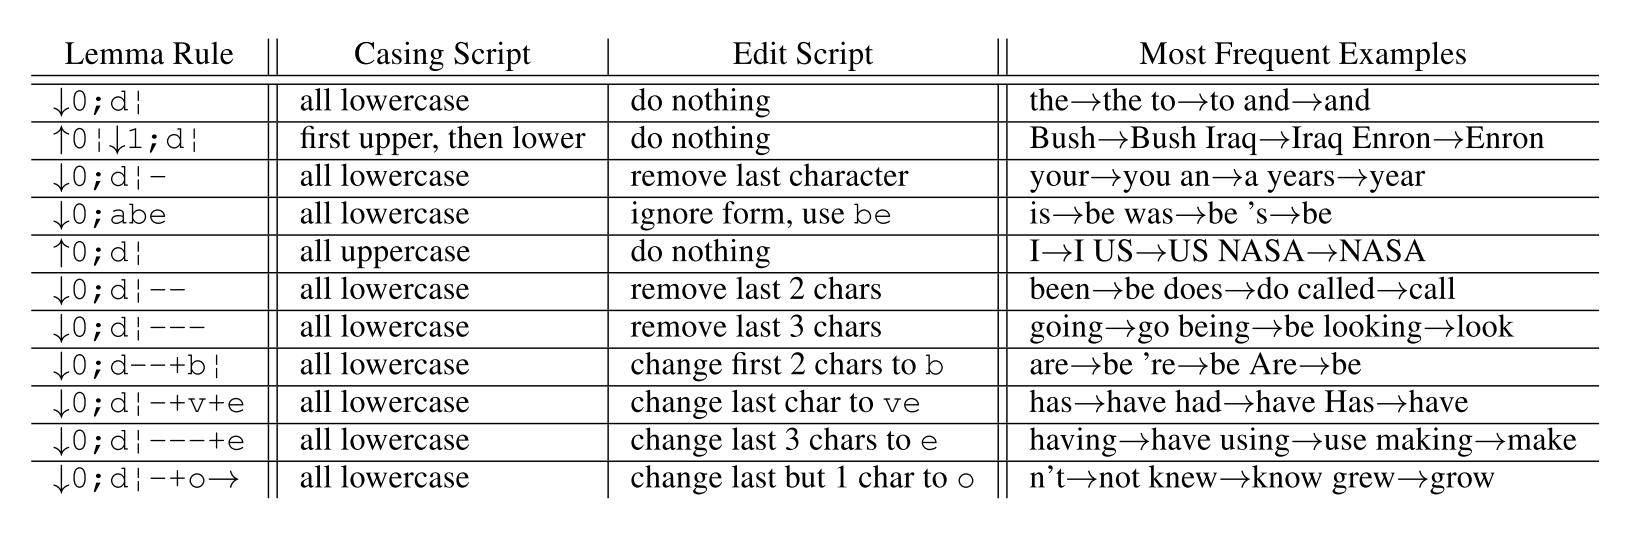
\includegraphics[width=1\textwidth]{../img/lemma_rules}
\protect\caption[The most common lemma generating rules in English EWT corpus]{
Table 1 from \citep{Straka2019b} presents 10 most common lemma generating rules in English EWT corpus. Each rule has two parts -- a casing script for transforming uppercase and lowercase letters, and an edit script. The edit script can transform prefix, suffix, or also a root of the word. It uses the Wagner–Fischer algorithm \citep{Wagner}, which finds the longest commont substring between the word and its lemma. Resulting rule is the shortest edit script converting the word into the lemma. More information can be found in \citep{Straka2019b}.
}
\label{fig:lemma_rules}
\end{figure}

\subsection{Related Work}
\subsubsection{Tagging}
This work aims to improve previously published SOTA results for contextualized embeddings in Czech lemmatization and tagging \citep{Straka2019} and \citep{Straka2021}. POS tagging (for English) is dated back to 1971 with first rule-based approach on Brown Corpus \citep{greene1971automatic}. Good results in POS tagging were achieved after year 2000 using both classical machine learning methods like Hidden Markov Models \citep{tnt} or Support Vector Machines \citep{svmtool}, and perceptrons/neural networks \citep{collins-2002-discriminative}. Actual English \acrshort{sota} known to me is presented in Flair model \citep{Akbik2018}.\footnote{More detailed overvirew of English tagging can be found here: https://aclweb.org/aclwiki/} It is necessary to note that early papers had \acrshort{pos} tagging defined differently than it is in this thesis. They focused only on selecting part of speech (noun, verb, etc...), meanwhile the later works (including this thesis) present complex morphological analysis.
\par
One of the first automatic tagging experiments in Czech is described in \citep{Hladka}, which also shows differences between languages with rich inflexion (as Czech,  but also Finnish or Turkish) and ones with simpler morphology (for example English or Spanish). Languages with complicated morphology have incomparably larger set of possible tags -- English has less then one hundred of possible tags, Czech has almost $4,000$ tags.  Current \acrshort{sota} results for tagging (and lemmatization) are presented in \citep{Straka2021}, which uses Czech version of RoBERTa model -- RobeCzech. This is the model also used for some experiments in this work and, as expected,  yields the best results. RobeCzech is based upon previous successful morphological analysis with contextual embeddings and BERT-like models \citep{Straka2019b}, \citep{Straka2019a}, \citep{Straka2019}, \citep{Straka2018} (all lastly mentioned models also achieved great results in lemmatization). \par
Although tagging is mostly considered to be a classification into predifined set of tags, the sets themselves can vary. Penn treebank uses a tagset of 54 different tags, which presents parts of speech and additional information like tense or number.\footnote{see: \url{https://www.sketchengine.eu/penn-treebank-tagset/}} There are some differences between this tagset and other English datasets or taggers (e.g., TreeTagger \citep{Schmid95improvementsin} or CLAWS tagset \citep{Chapelle1988TheCA}). All English tagsets are really small compared to languages like Czech or Turkish. As mentioned before, Czech uses 15-positioning tags, which is a natural solution for such type of languages. These positions can be predicted together or for each position separately. The first approach creates big tagset but guarantees consistency among positions (e.g. there will be no tense for a noun or a case for a verb). In the case of separate prediction, each position can be treated as a classification problem separately, which causes problems, because the individual parts of tag are not independent. Better approach is to use sequence-to-sequence modelling \citep{Sutskever2014}, which outputs the tag as a sequence of positions and takes into account previously generated position as in \citep{malaviya-etal-2019-simple}.

\subsubsection{Lemmatization}
Lemmatization (both Czech and English) has undergone a similar development as tagging, starting with rule-based approaches and statistical approaches \citep{Plisson}, continuing with neural networks and recently achieving good results with BERT-like models \citep{Kondratyuk2019}.  Lemmatization is typically performed as a sequence-to-sequence model, therefore it takes a word as a sequence of characters and produces a new sequence of characters, which is the lemma. This approach is teoretically better than classification into rules, because it is possible to generate every existing lemma. However, it can generate simply every possible character sequence, which may not be an existing word. Lemmatization as a classification task into edit scripts set firstly appeared in \citet{Chrupala} and was explored further by \citet{Straka2018}. 
Sequence-to-sequence model can be also used for production of edit rules (same rules as used in this work)\citep{chakrabarty2017context}, \citep{muller2015joint} and \citep{Yildiz2019}.

\subsection{Dataset and Preprocessing}
\label{sub:dataset}
Dataset for these tasks is taken from data of Prague Dependency Treebank (PDT) \citep{PDT35}, version 3.5 from year 2018. Data consists of sentences with lemmas and tags. For ambiguous words, data contain all possible analyses, which were generated using morphoDita \citep{Strakova} and morphological dictionary \citep{11234/1-1834} (described later).\footnote{genarator of analyses is available online: \url{https://lindat.mff.cuni.cz/services/morphodita/}.} For example, Czech word "psa" has one possible lemma ("pes") but two possible tags, because it could be one of two possible grammatical cases -- genitive or accusative. Input data for such word looks as follows: \\
\begin{center}
\texttt{psa pes NNMS2-----A---- NNMS4-----A----}.
\end{center}
Data contains about 1,600 unique tags and about 1,500 different lemma rules. The number of lemmas is significantly smaller than a number of unigue lemmas ($72,000$) \citep{Strakova} or tags, because words with similar morphological function have same way of creating lemma from the word, e.g. words \textit{malého} (=little, accusative,  sg, m.,) and \textit{červeného}  (=red, accusative,  sg, m.,) have the same lemma rule:
\begin{center}
\texttt{$\downarrow$ 0;d\textbrokenbar ---+ý+-+1}.
\end{center} 
\par
Dataset is originally divided into tree parts - train, development and test, which is also used in this work. Input sentences are preprocessed as follows:
\begin{itemize}
\item mapping characters and words into numbers -- Mapping  words/characters, which were found in train dataset into integers (from one to the number of unique words). This means that the network has no information about words/characters which appears only in test or development dataset. All newly appeared words/characters are mapped into one same number (typically $0$) for \textit{UNK} token/character.
\item tokenization -- Tokenizer for corresponding BERT-like model transforms input words into tokens. Each word is transformed into one or more strings, which are converted into numbers. This serves as an input into BERT part of the model. To create these input embeddings, the whole sentence for each word is needed as the same words can have different representation in different contexts. More information can be found in section \ref{sub:tokens}.
\end{itemize}

\subsection{Architecture and Experiments}

\begin{figure}[!h]
\centering
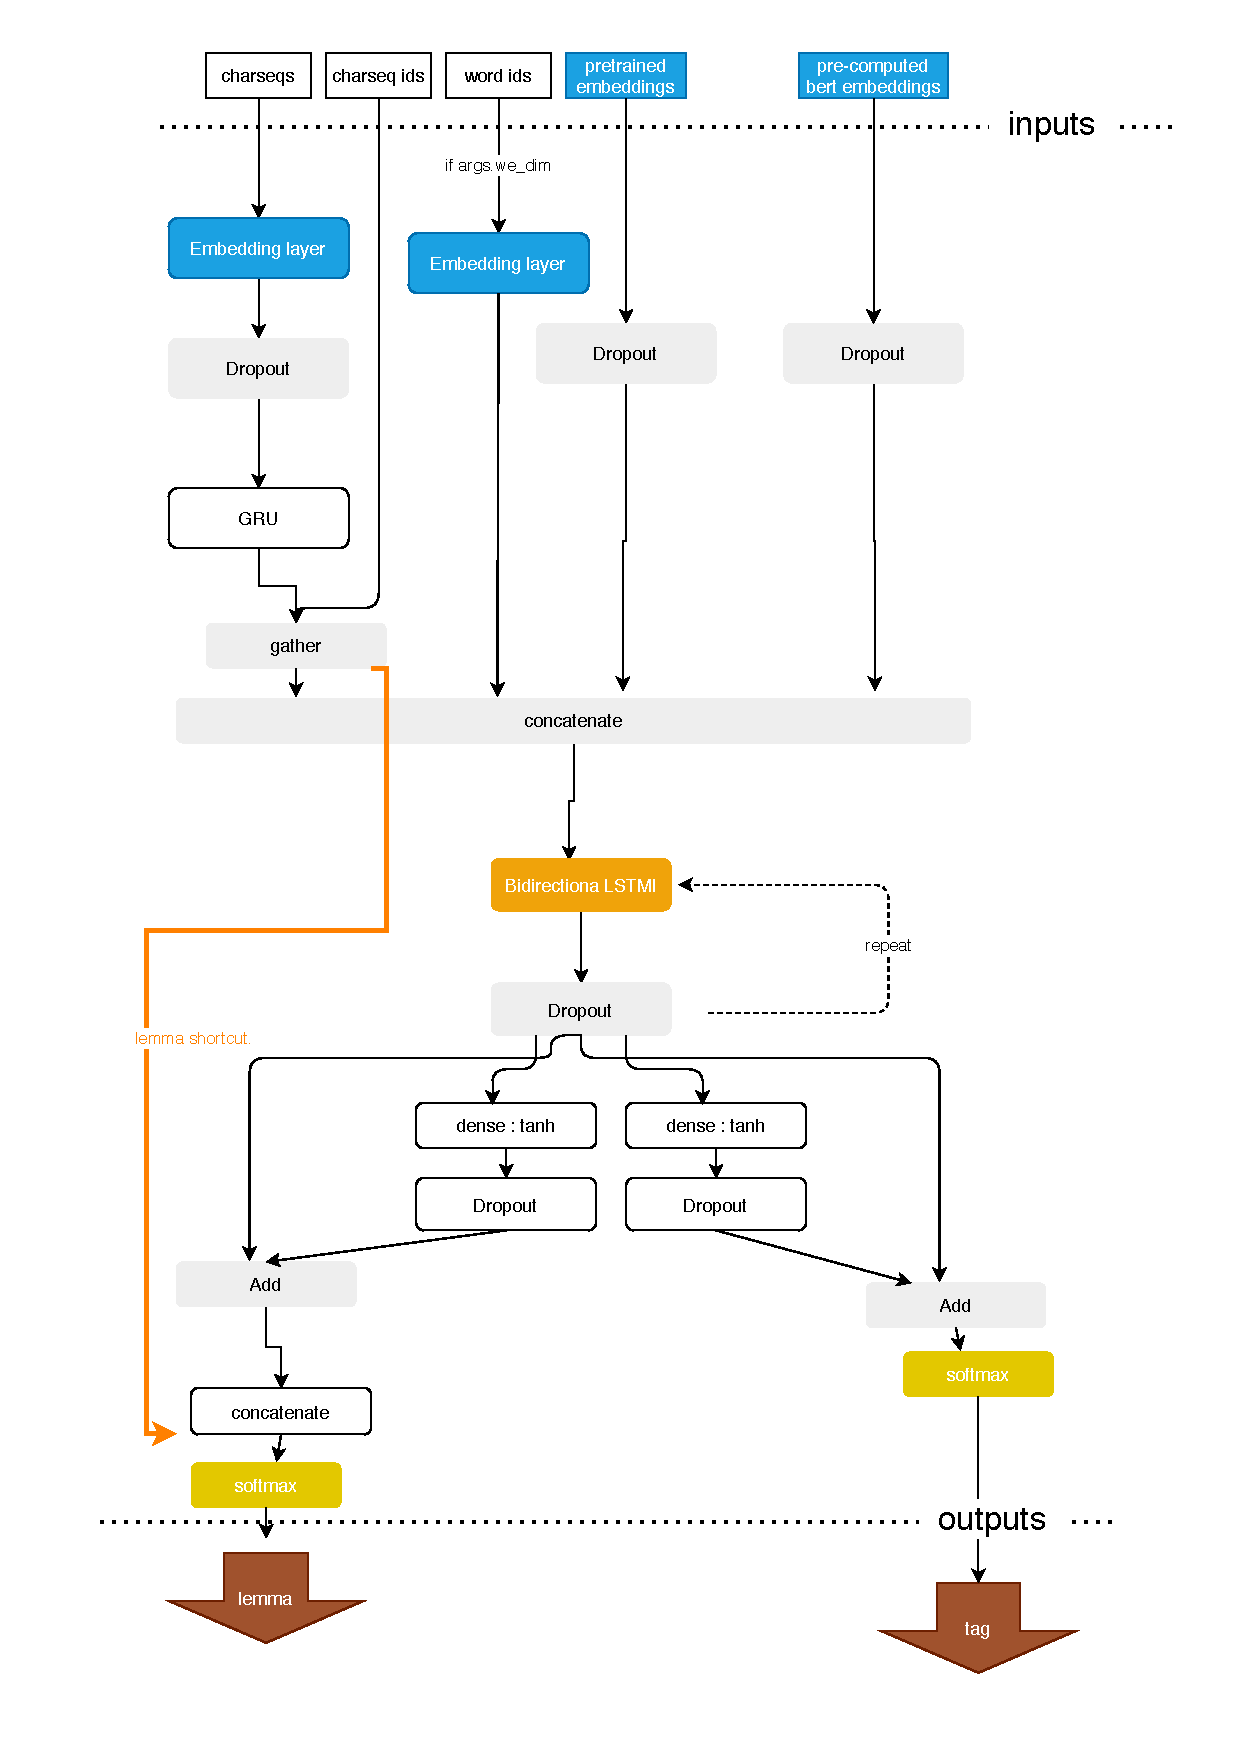
\includegraphics[width=1\columnwidth]{../img/taggermodel.pdf}
\protect\caption{Tagging and lemmatization joint model architecture.}
\label{pic:lt_arch}
\end{figure}
%TODO kolik je tech lstm a tak,vsechny dimenze (do tabulky)

%For POS tagging, we applied a straightforward model in the lines of Ling et al. (2015) – first rep- resenting each word with its embedding, contextu- alizing them with bidirectional RNNs (Graves and Schmidhuber, 2005), and finally using a softmax classifier to predict the tags. z UDpipe2

The model for lemmatization and tagging is build upon a model (and a code) for previous work on Czech NLP processing with contextual embedding \citep{Straka2019}. 
Data preprocessing is taken over from the paper as well as the structure of the lemmatizer and the tagger network, which is extended by BERT-like models, hoping for improvements. %TODO k tomu nemam citaci
Previous work showed that training tagging and lemmatization together in one network can be mutually advantageous, so both of these analyses are an output of one network, and are trained jointly. Detailed visualisation of network architecture can be found in figure \ref{pic:lt_arch}. \par The architecture of the network can be divided into three parts -- inputs, optional \acrshort{rnn}s, classification head:
\paragraph{Inputs}
An input set of the network consists of five different input types -- characters (charseqs), words (charseq ids), correct responses (word ids), pretrained embeddings, and possibly precomputed BERT embeddings (depending on the experiment type). Two other types of embeddings are created before the further processing of inputs by \acrshort{rnn} cells: character-level embeddings and another word embeddings that are, in contrast to BERT and pretrained embeddings, also trained during the training process.

\paragraph{RNN cells}
Character-level embeddings are further processed via 1 layer of \acrfull{gru} and all inputs (or their embeddings) are processed by recurrent part of network (specifically by three layers of \acrfull{lstm} cells).

\paragraph{Classification head(s)}
After the processing by recurrent neural networks, network employs two separate classification heads, one for tagging and another for lemmatization. Both heads use dense layer with tanh activation function to allow task-specific non-linear transformation as used in \citep{Straka2018} and a softmax function for obtaining the probability distribution over target classes. Lemmatization, however, presents another change -- addition of character level data without RNN processing, that are used together with the rest of the values as an input into the softmax following \citep{Straka2018}, as it leads to better performance of lemmatization in the case of shared network between both tasks.

%TODO kondraytuk bere predikci k prvnímu subwordu, jak to delam ja? 


\paragraph{Morphological Dictionary} All classification can be done with or without use of a morphological dictionary MorfFlex \citep{11234/1-1834}, that can provide possible pairs \textit{tag-lemma}. If used, the generated tag and lemma is a pair with maximal likelihood, but chosen just from the dictionary. This leads to more consistent results. 

%TODO maximal probability



%TODO nekde mam taky dropouts! zminit
\subsubsection{Experiments}
This part uses all main \textbf{experiment types} as decribed in \ref{sec:expe}: \textit{base, ls, embed, fine, simple}, and \textit{full}. Three \textbf{BERT-like models} are used for experiment setup:
\begin{itemize}
\item multilingual BERT (mBERT) \citep{Devlin2019}, 
\item XLM-RoBERTa \citep{Conneau2019}, 
\item RobeCzech \citep{Straka2021}.
\end{itemize}
XLM-RoBERTa and mBERT are trained on 100/104 different languages including Czech. RobeCzech is a recently published version of RoBERTa, trained only on Czech data. XLM-RobERTa is used only for embedding and one version of fine-tuning, and this model was omitted in other experiements because of weak results and high computational complexity. There exists another monolingual Czech model, Czert \citep{Sido2021}, which uses the original BERT architecture and was outperformed by RobeCzech \citep{Straka2021}. \par
A selection of layers is made in both ways -- last four layers (\textit{four)} and learning of weighted sum of all layers (\textit{att}). The layer attention is made only for the fine-tuning setup, and as the weighted sum does not show a significant benefit, mean of the last four layer is the only method used for other experiments.
 \par Learning rate is used as usual for each type of task and three different learning rate schedules were applied in each combination of hyperparameters: cosine decay \textit{(cos)}, inverted square root decay \textit{(isrd)} and a one epoch warm-up followed by a constant learning rate \textit{(warmup)} inspired by \citep{Kondratyuk2019} and \citep{Ruder2018}. For \textit{embed} experiments, \textit{warmup} is replaced by  a simple division of training into two parts with different learning rates. 
 
 \begin{table}[!h]
 \centering
\begin{tabular}{|l||l|}
\hline
hyperparametr   & \multicolumn{1}{l|}{value} \\ \hline \hline
beta\_2          & 0.99                       \\ \hline
optimizer       & Adam                       \\ \hline
cle\_dim         & 256                        \\ \hline
dropout         & 0.5                        \\ \hline
label smoothing & 0.3                        \\ \hline
rnn\_cell        & LSTM                       \\ \hline
rnn\_cell\_dim    & 512                        \\ \hline
rnn\_layers      & 3                          \\ \hline
we\_dim          & 512                        \\ \hline
word\_dropout    & 0.2                        \\ \hline
batch size & 64 \\ \hline
\end{tabular}
\caption[Hyperparameters of tagging and lemmatization common to all experiments]{Hyperparameters of tagging and lemmatization common to all experiments (if they make sense in the context of experiments).}
\label{tab:hyp_all}
\end{table}
Batches have size 64, given by the compromise between the pursuit of relatively big batch size and computational resources. Summary of hyperparameters, which do not differ across experiments is presented in table \ref{tab:hyp_all}. Other hyperparameters for each experiment are in table \ref{att:1}.
\par 
Reimplementation of \citep{Straka2019a} without any BERT-like model incorporation serves as a baseline.

\subsection{Results and Discussion}
Best presented model (experiment no. 18) achieved the same or better results than the current \acrlong{sota} tagging and lemmatization results (table \ref{tab:all_prew}). Complete results are in table \ref{tab:all_res_tl}. Experiment \textit{tl\_18} is the version with fine-tuning, Czech monolingual model, RobeCzech, and without layer attention, although the difference from comparable experiment with layer attention is insignificant and can be just accidental. The dominance of the Czech model was expected and additional expert knowledge contained in the complicated architecture was also assumed to be better. Experiments also showed that fine-tuning approach achieves better results than full training from the beginning. This may be due to the choice of hyperparameters, especially the learning rate, but the standard ones were selected, implying that at best, it is more difficult to find the right parameters for\textit{full} and \textit{simple} variants. Although \textit{simple} experiments presents standard approach of using pretrained BERT models, they turned out being less successful even than \textit{embed} experiments, that are faster to train and less memory intensive. 

\begin{table}[!h]
\centering
  \resizebox{\columnwidth}{!}{\begin{tabular}{|l||ccc||ccc|}
  \hline
\multirow{2}{*}{Experiment} & \multicolumn{3}{c||}{Without Dictionary}  &
      \multicolumn{3}{c|}{With Dictionary} \\ 
    & Tags & Lemmas & Both & Tags & Lemmas & Both \\ \hline \hline
    \textit{\citep{Straka2019}} & \textit{97.94} & \textit{98.75} & \textit{97.31} & \textit{98.05} & \textit{98.98} & \textit{97.65 }\\ \hline
   \textit{ StrakaC} & \textit{97.67} & \textit{98.63} & \textit{97.02} & \textit{97.91 }& \textit{98.94} & \textit{97.51} \\ \hline
     \textit{RobeCzech} & \textit{98.43} & \textit{98.79}  & \textit{97.83}  & \textit{98.50} & \textit{\textbf{99.00}}  & \textit{98.11} \\ \hline \hline
      baseline & 97.04  & 98.56  & 96.41 &  97.31   & 98.83  & 96.90 \\ \hline 
    emb(12) & 98.38  &98.79  & 97.80 & 98.48  & 98.99 & 98.10 \\ \hline
    best(18) & \textbf{98.50}  & \textbf{98.80} &\textbf{ 97.90}  & \textbf{98.57}  & \textbf{99.00}  & \textbf{98.19}  \\ \hline  
  \end{tabular}}
  \caption[Comparison of our best results and previous work]{
  \textit{Straka2019C} is a comparable solution  (BERT embeddings only) from \citep{Straka2019} to \textit{emb}, which was transformed into Tensorflow 2 in this work as a \textit{baseline}. \textit{Emb} is a solution with static BERT embeddings and \textit{best(18) is the best resulting model in this thesis (experiment id = 18). }}
\label{tab:all_prew} 
\end{table}


%TODO vsechny Figure a table se stejnym pismenem

\begin{table}[!h]
\resizebox{\columnwidth}{!}{
\begin{tabular}{|l|l|l|l|l|l||llllll|}
\hline
\multicolumn{2}{|c|}{\multirow{2}{*}{Model}} &
  \multirow{2}{*}{EXPE} &
  \multirow{2}{*}{EP} &
  \multirow{2}{*}{LAYERS} &
  \multirow{2}{*}{LR} &
  \multicolumn{2}{c}{Lemmas} &
  \multicolumn{2}{c}{Tags} &
  \multicolumn{2}{c|}{Both} \\
\multicolumn{2}{|l|}{} &  &  &  &  & Raw & Dict & Raw & Dict & Raw & Dict  \\ \hline \hline
0  & NA                           & base                    & A	& NA               & simple & 98.58  & 98.81   & 97.05   & 97.31    & 96.43     & 96.9       \\ \hline
1  & NA                           & ls                      & B	& NA               & simple & 98.55  & 98.81   & 97.12   & 97.34    & 96.51     & 96.94      \\ \hline
2  & \multirow{3}{*}{mBERT}       & \multirow{9}{*}{embed}  & B	& four             & simple & 98.69  & 98.93   & 97.83   & 97.98    & 97.17     & 97.58      \\ \cline{1-1} \cline{4-12}
3  &                              &                         & C	& four                     & cos    & 98.74  & 98.95   & 97.91   & 98.04    & 97.28     & 97.63      \\ \cline{1-1} \cline{4-12}
4  &                              &                         & C	& four                     & isrd   & 98.73  & 98.94   & 97.89   & 98.02    & 97.28     & 97.61      \\ \cline{1-2} \cline{4-12}
5  & \multirow{3}{*}{xlm-Roberta} &                         & B	& four             & simple & 98.57  & 98.8    & 97.33   & 97.54    & 96.68     & 97.12      \\ \cline{1-1} \cline{4-12}
6  &                              &                         & C	& four                     & cos    & 98.6   & 98.83   & 97.45   & 97.62    & 96.81     & 97.21      \\ \cline{1-1} \cline{4-12}
7  &                              &                         & C	& four                     & isrd   & 98.59  & 98.83   & 97.44   & 97.61    & 96.81     & 97.2       \\ \cline{1-2} \cline{4-12}
8  & \multirow{3}{*}{RoBECzech}   &                         & B	& four             & simple & 98.77  & 98.97   & 98.38   & 98.48    & 97.78     & 98.08      \\ \cline{1-1} \cline{4-12}
9  &                              &                         & C	& four                     & cos    & 98.79  & 98.99   & 98.38   & 98.48    & 97.80      & 98.10      \\ \cline{1-1} \cline{4-12}
10 &                              &                         & C	& four                     & isrd   & 98.78  & 98.98   & 98.4    & 98.48    & 97.8      & 98.09      \\ \hline
11 & \multirow{3}{*}{mBERT} & \multirow{9}{*}{fine}         & D	& four     & simple & 98.69 & 98.93 & 97.84 & 97.99 & 97.21 & 97.59 \\ \cline{1-1} \cline{4-12}
12 &                              &                         & E	& four             & cos    & 98.72  & 98.95   & 97.97   & 98.08    & 97.33     & 97.68      \\ \cline{1-1} \cline{4-12}
13 &                              &                         & E	& four             & isrd   & 98.68  & 98.9    & 97.72   & 97.86    & 97.09     & 97.46      \\ \cline{1-2} \cline{4-12}
14 & \multirow{3}{*}{xlm-Roberta} &                         & D	& four     & simple & 98.62  & 98.84   & 97.72   & 97.9     & 97.07     & 97.48      \\ \cline{1-1} \cline{4-12}
15 &                              &                         & E	& four             & cos    & 98.67  & 98.9    & 97.95   & 98.09    & 97.32     & 97.69      \\ \cline{1-1} \cline{4-12}
16 &                              &                         & E	& four             & isrd   & 98.63  & 98.85   & 97.66   & 97.83    & 97.03     & 97.41      \\ \cline{1-2} \cline{4-12}
17 & \multirow{3}{*}{RoBECzech}   &                         & D	& four     & simple & 98.78  & 98.98   & 98.46   & 98.55    & 97.86     & 98.16      \\ \cline{1-1} \cline{4-12}
18 &                              &                         & E	& four             & cos    & \textbf{98.80}   & \textbf{99.00 }     & \textbf{98.50}    & \textbf{98.57}    & \textbf{97.90 }     & \textbf{98.19 }     \\ \cline{1-1} \cline{4-12}
19 &                              &                         & E	& four             & isrd   & 98.76  & 98.95   & 98.33   & 98.41    & 97.72     & 98.02      \\ \cline{1-2} \cline{4-12} \hline
20 & \multirow{3}{*}{mBERT}  &  \multirow{9}{*}{fine att}   & D	& att                       & simple & 98.67  & 98.91   & 97.76   & 97.92    & 97.13     & 97.52      \\ \cline{1-1} \cline{4-12}
21 &                              &                         & E	& att              & cos    & 98.72  & 98.95   & 97.98   & 98.1     & 97.34     & 97.69      \\ \cline{1-1} \cline{4-12}
22 &                              &                         & E	& att              & isrd   & 98.67  & 98.91   & 97.69   & 97.85    & 97.05     & 97.45      \\ \cline{1-2} \cline{4-12}
23 & \multirow{3}{*}{xlm-Roberta} &                         & D	& att      & simple & 98.6   & 98.81   & 97.62   & 97.77    & 96.96     & 97.35      \\ \cline{1-1} \cline{4-12}
24 &                              &                         & E	& att              & cos    & 98.67  & 98.89   & 97.91   & 98.06    & 97.29     & 97.66      \\ \cline{1-1} \cline{4-12}
25 &                              &                         & E	& att              & isrd   & 98.65  & 98.86   & 97.65   & 97.81    & 97.03     & 97.41      \\ \cline{1-2} \cline{4-12}
26 & \multirow{3}{*}{RoBECzech}   &                         & D	& att      & simple & 98.77  & 98.97   & 98.38   & 98.47    & 97.79     & 98.08      \\ \cline{1-1} \cline{4-12}
27 &                              &                         & E	& att              & cos    & \textbf{98.8}   & 98.99   & 98.47   & 98.54    & 97.88     & 98.16      \\ \cline{1-1} \cline{4-12}
28 &                              &                         & E	& att              & isrd   & 98.77  & 98.96   & 98.33   & 98.41    & 97.72     & 98.01      \\ \hline
29 & \multirow{3}{*}{mBERT}       & \multirow{9}{*}{simple} & F	& four                     & warmup & 98.17  &         & 97.32   &          & 96.46     &            \\ \cline{1-1} \cline{4-12}
30 &                              &                         & G	& four                     & cos    & 98.15  &         & 97.39   &          & 96.47     &            \\ \cline{1-1} \cline{4-12}
31 &                              &                         & G	& four                     & isrd   & 98.13  &         & 97.12   &          & 96.29     &            \\ \cline{1-2} \cline{4-12}
35 & \multirow{3}{*}{RoBECzech}   &                         & F	& four                     & warmup & 98.49  &         & 98.28   &          & 97.41     &            \\ \cline{1-1} \cline{4-12}
36 &                              &                         & G	& four                     & cos    & 98.46  &         & 98.30   &          & 97.39     &            \\ \cline{1-1} \cline{4-12}
37 &                              &                         & G	& four                     & isrd   & 98.59  &         & 98.27   &          & 97.53     &            \\ \hline
38 & \multirow{3}{*}{mBERT}       & \multirow{9}{*}{full}   & F	& four                     & warmup & 98.16  & 98.86   & 97.35   & 97.79    & 96.46     & 97.34      \\ \cline{1-1} \cline{4-12}
39 &                              &                         & G	& four                     & cos    & 98.04  & 98.85   & 97.36   & 97.81    & 96.3      & 97.34      \\ \cline{1-1} \cline{4-12}
40 &                              &                         & G	& four                     & isrd   & 98.22  & 98.86   & 97.34   & 97.73    & 96.46     & 97.29      \\ \cline{1-2} \cline{4-12}
44 & \multirow{3}{*}{RoBECzech}   &                         & G	& four                     & warmup & 98.49  & 98.95   & 98.21   & 98.34    & 97.38     & 97.93      \\ \cline{1-1} \cline{4-12}
45 &                              &                         & G	& four                     & cos    & 98.25  & 98.95   & 98.17   & 98.33    & 97.08     & 97.89      \\ \cline{1-1} \cline{4-12}
46 &                              &                         & G	& four                     & isrd   & 98.55  & 98.99   & 98.19   & 98.35    & 97.39     & 97.95      \\ \hline

\end{tabular}
}
\caption[Complete results for tagging and lemmatization]{This table presents complete results for tagging and lemmatizationt tasks. Column EP presents number of epochs and corresponding learning rates are explained in Attachement \protect\ref{att:1} }
\label{tab:all_res_tl}
\end{table}

\subsubsection{Error Analysis}
%TODO sjednotit názvy modelů
This section offers a little exploration of differences in error across models. This comparison includes three models: 
\begin{itemize}
\item tl\_18 -- the best model in tagging and lemmatization,
\item tl\_3 -- the best model with mBERT,
\item tl\_1 -- the baseline model with label smoothing.
\end{itemize} 

\paragraph{best vs. baseline}
The best model (tl\_18) improves prediction in $3,247$ tags and is worse in 421 tag predictions. More than 80\% of newly correctly predicted tags are composed by three parts of speech: NN (noun), AA (adjective), and RR (preposition). Table \ref{att:tags1} presents improved tags with a frequency at least 10. The most frequent tag ( \texttt{NNIS1-----A----}) presents proper names of places (e.g. Jersey, Tenesee), but we can see that other frequent tags are nominatives and accusatives of masculinum, singular,  inainamate (cs: \textit{rod mužský neživotný}) or femininum, plural. These two cases have the same form for mentioned categories, so they are indistinguishable without context, and that is where BERT showed to be very useful. The same situation is with adjectives, again mostly nominative or accusative of the same form, for example words \textit{další} (following) or \textit{stínový} (shadowy). The third category are prepositions that can be connected with both accusative and dative as \textit{na} (on), or \textit{o} (about).

%TODO kolik lemmata

\paragraph{mBERT vs. RobeCzech}
Best mBERT is better in 468 tags and worse in $1,703$ tags than the best model. The most frequent tags improved by \textit{tl\_18} are similar to previous comparison. Nominative and accusative are again the most common cases improved, but the differences between these two models are not so significant. This results in verbs appearing higher in the table of most frequent tags, although the absolute value of better predictions on verbs is similar to previous comparison. In both situations, improved verbs predictions relate mostly to verbs with the same form in singular and plural of the third-person, e.g. \textit{vyváží} (exports) or \textit{stojí} (stands). The complete table of the most frequent tags is available in table \ref{att:tags2}.
%TODO kolik lemmata
%TODO je v necem mBERT lepsi?

\newpage
\section{Sentiment Analysis}
\label{chap:sent}
As stated in \citep{Veselovska}: "Sentiment analysis, also known as opinion mining, is an automatic detection of a positive or negative polarity, or neutrality of ... a text sequence", which is exactly as the sentiment analysis is understood in this work, although there are some other definitions consisting of e.g. opinion extraction, irony or stance \citep{Montoyo2012}. Another tasks related to sentiment analysis is a subjectivity analysis (whether the presented opinion is objective or highly subjective), which is also not included in this work, mainly because the lack of labelled data for Czech. It is possible to analyze individual expressions, sentences or whole documents \citep{Veselovska} and this work focuses on the document level classification.
\subsection{Task definition}
\paragraph{Sentiment analysis} \mbox{}\\
\textit{input:} sequence of sentences (a whole post or comment, depending on the source) \\
\textit{output:} prevailing sentiment of the input from categories: neutral, positive, negative.
\par

\paragraph{Metric} For evaluating performance, two metrics are used: macro-averaged F1 score and accuracy. Both metrics are chosen for better comparability with previous work.

\subsection{Related Work}
citace:
\citep{Cano2019}
\citep{Kittask2020} .. estonian
\citep{Lenc2016} sentiment in czech
\citep{Hercig2018}
\citep{Li}
\citep{Libovicky} presents state-of-the art results in three czech NLP tasks including sentiment analysis. They use only CSFD dataset with resulting accuracy 80.8 .1 which is still not so good as Brychcín (81.5.3). The second mentioned paper, however, uses quite complicated method for classification incorporating the fact of which movie is reviewed. 

Bachelor thesis which aplies bert on sentiment analysis in czech:
%https://dspace.cvut.cz/bitstream/handle/10467/83127/F8-BP-2019-Langr-Lukas-thesis.pdf?sequence=-1&isAllowed=y
results are accuracy 84 with tfidf and about 81 with bert and they used mall dataset.

\subsection{Dataset and Preprocessing}
%TODO zjistit jaka jsou na to porovnavaci data This work primary tries to improve existing tasks and show the ability of contextualized embeddings to improve results, so tasks with existing data and results were selected.  %TODO why?
Four main Czech datasets with sentiment annotation are available: user reviews from MALL.cz (mall), film reviews from csfd.cz (csfd), news from Aktualne.cz (aktualne) and posts from czech branch pages on facebook.cz (facebook). As \textit{aktualne} dataset turned out to be problematical because the text were ambiguous even for annotators, and its authors later used other mentioned datasets \citep{Veselovska}, this work also focuses only on the three other data sources -- \textit{mall}, \textit{csfd} and \textit{facebook} \footnote{All three datasets are all available here: http://liks.fav.zcu.cz/sentiment/}. Some experiment are also performed with in-domain training on Eglish data. For this purpose is used \textit{imdb} dataset \footnote{https://www.tensorflow.org/datasets/catalog/imdb\_reviews}, which contains movie review from the biggest movie rating website imdb.com. This leads to some problems described later in this section, because English dataset contains only binary classification (positive/negative). Table \ref{tab:datasets} summarize each dataset.
%TODO popis tabulky
\begin{center}
\begin{table}[]
\begin{tabular}{|l||lll|}
\hline
     & length & labels                                                                & domain        \\ \hline \hline
\textbf{mall}     & 145306 & \begin{tabular}[c]{@{}l@{}}positive\\ neutral\\ negative\end{tabular} & domestic appliance reviews                             \\ \hline
\textbf{csfd} & 91304  & \begin{tabular}[c]{@{}l@{}}positive\\ neutral\\ negative\end{tabular} & movie reviews \\ \hline
\textbf{facebook} & 9752   & \begin{tabular}[c]{@{}l@{}}positive\\ neutral\\ negative\end{tabular} & \begin{tabular}[c]{@{}l@{}}brand pages of e.g. shops or mobile networks \\ providers\end{tabular} \\ \hline
\textbf{imdb} & 25000  & \begin{tabular}[c]{@{}l@{}}positive\\ negative\end{tabular}           & movie reviews \\ \hline
\end{tabular}
\label{tab:datasets}
\caption{Three Czech datasets (mall, facebook, csfd) and one English (imdb) are used for training in this work.}
\end{table}
\end{center}


%TODO je to rozdleeno se stratifikací?
%TODO popis obrazku
\begin{figure}[!ht]
\centering
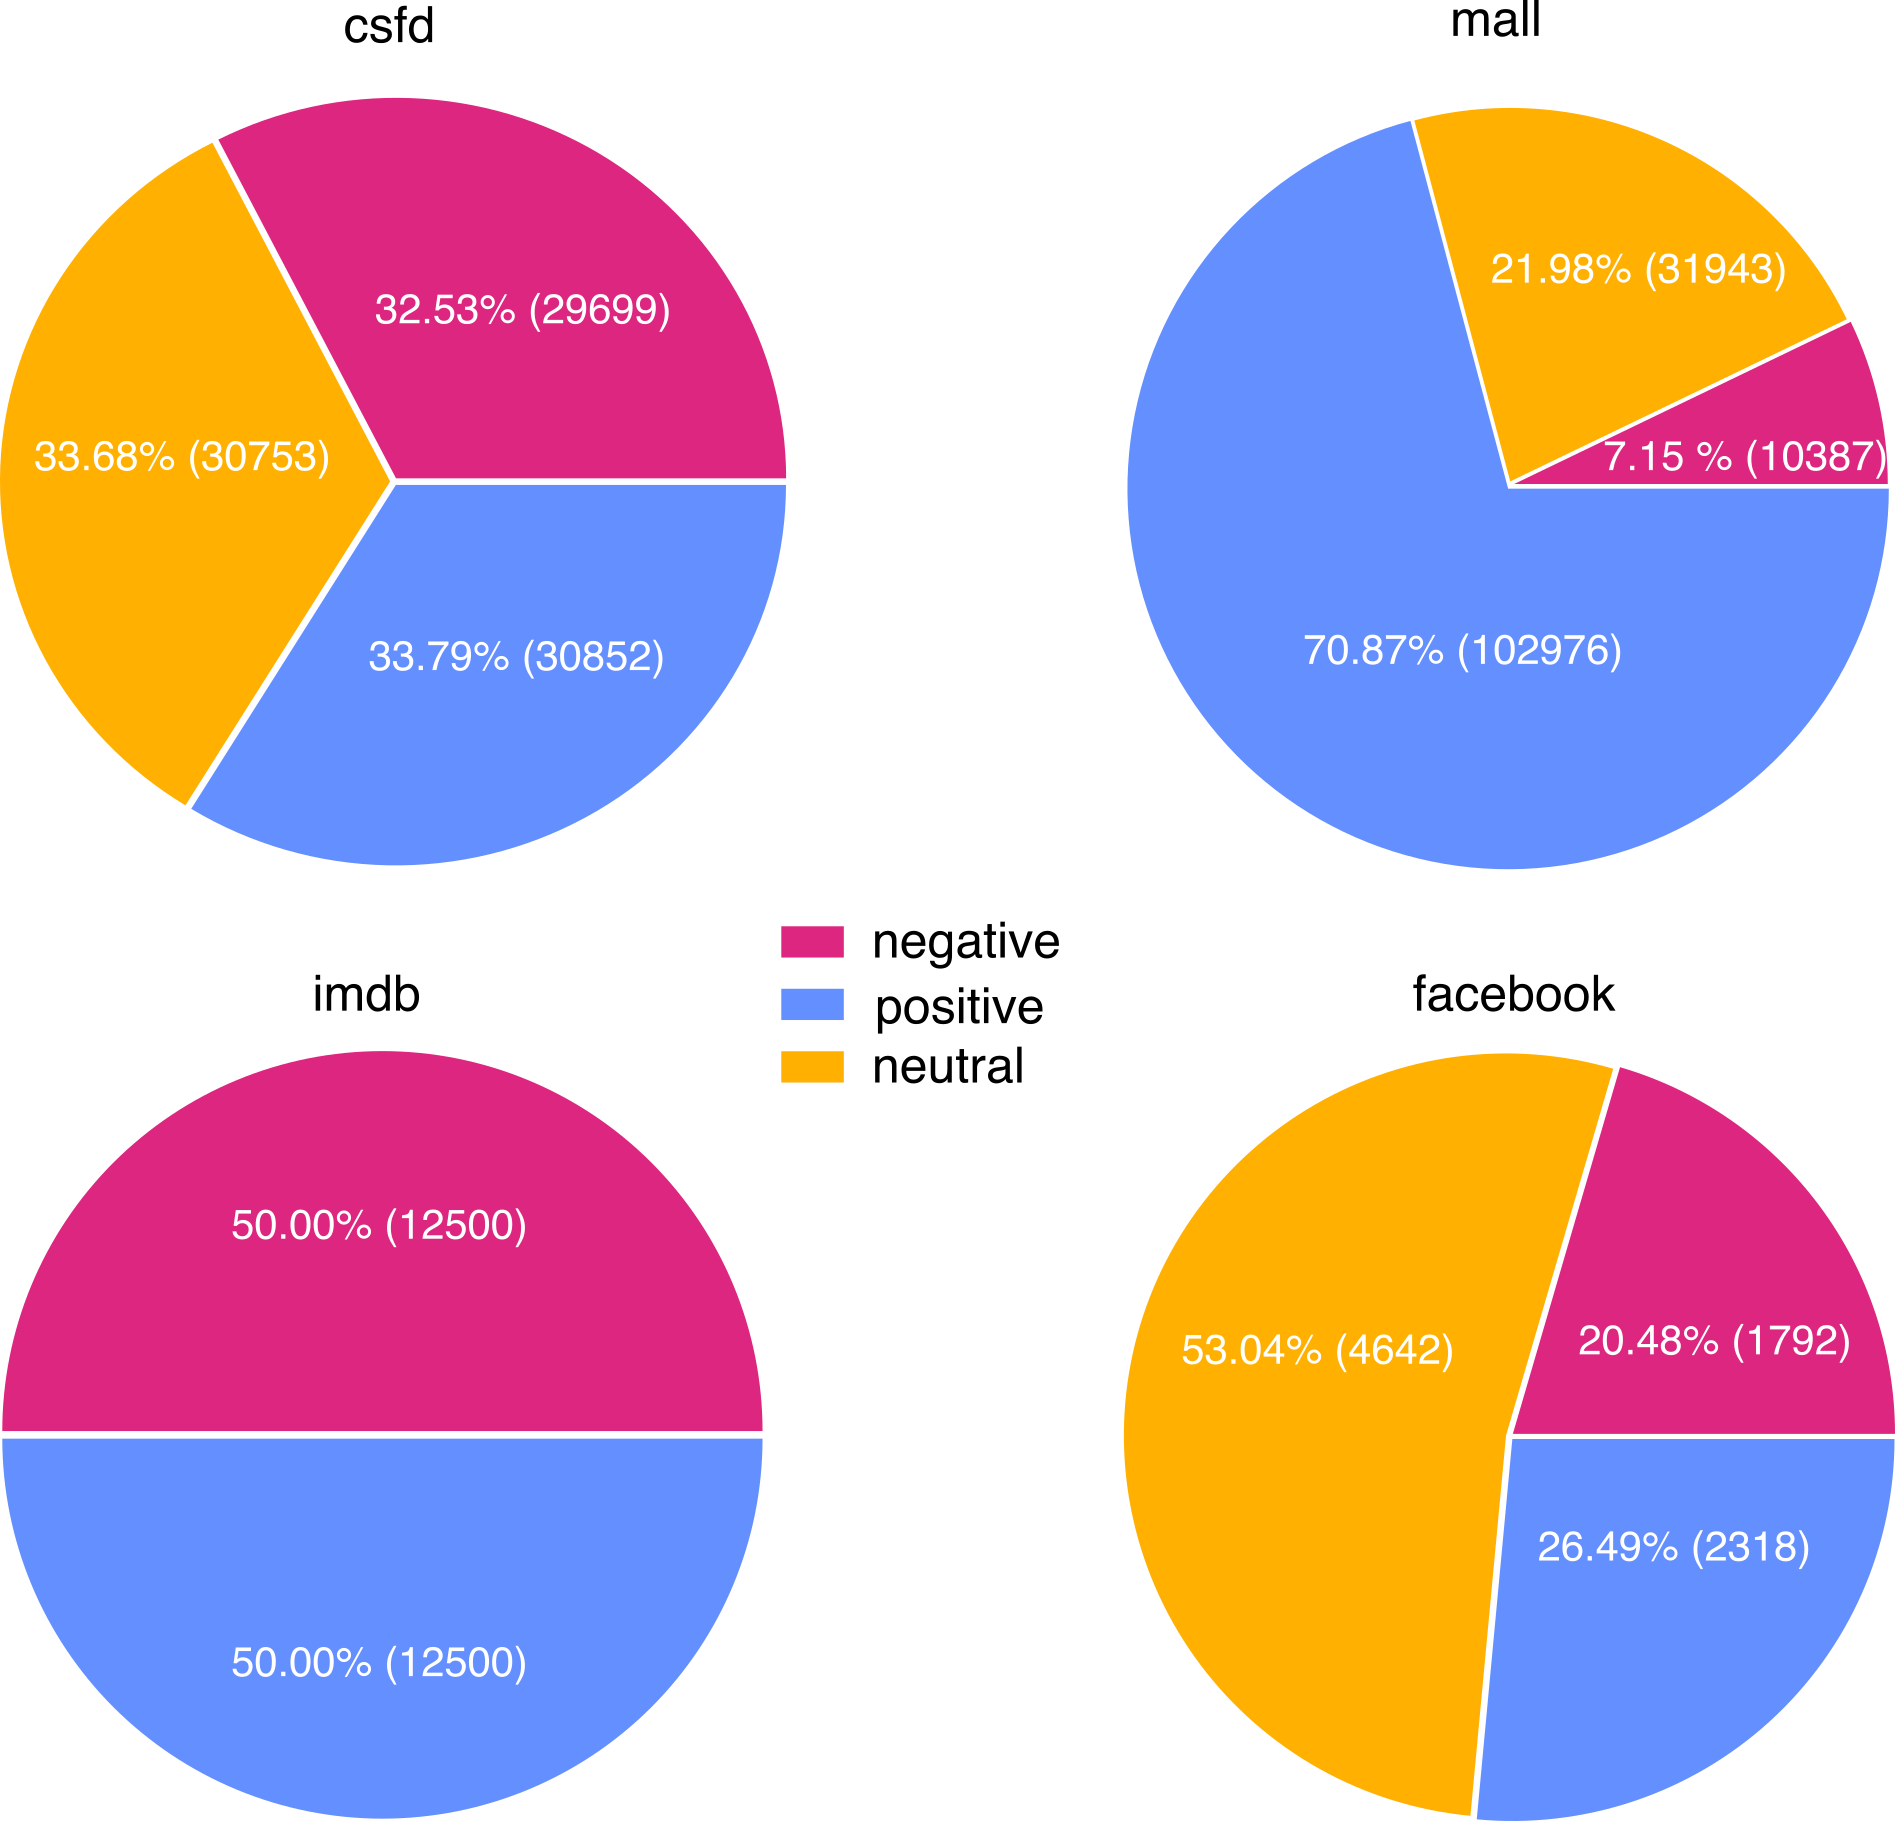
\includegraphics[width=1\columnwidth]{../img/dist_all.png}
\protect\caption{Distribution of positive/neutral/negative labels in each dataset.}
\label{pic:dist}
\end{figure}

As can be seen in figure \ref{pic:dist}
distribution of labels differs among datasets. Moreover, Figure \ref{pic:dist_all}
\begin{figure}[!ht]
\centering
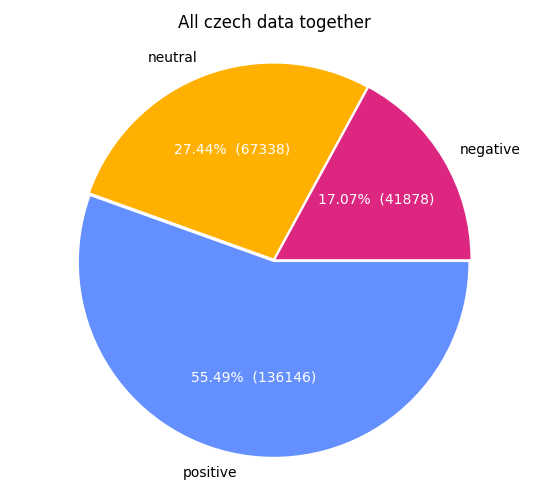
\includegraphics[width=0.7\columnwidth]{../img/all.png}
\protect\caption{Percentage and absolute values of labels in all three Czech datasets together.}
\label{pic:dist_all}
\end{figure}
%TODO all má blbý nadpis
shows, that the resulting dataset is highly unbalanced, which causes divergence and stuck in training. Due to the big part of labels being positive, many learning strategies just ended with predicting only \textit{positive} class, i.e. 55\% accuracy, so unfortunately learned nothing. 

%This was the the case for following experiments settings:
%learning rate of $2e-3$ for 10 epochs. This ended with predicting only one class (positive). Some progress showed the followign approach:"2:5e-5,1:2e-5, unfreezed" for facebook data only (which are balanced). This results are above 71 for accuracy (Test accuracy: 0.726
%F1 metrics: 0.7077061630227595 weighted).


\subsection{Experiments and Architecture}
The main division of experiments is by the input dataset -- each of Czech models separately and one joint dataset consisting of all Czech datasets, i.e. four different datasets. All variants performed both layers attention and an average of last four layers. As for the learning rate, all experiments were made with learning rate $3 \times 10^{-5}$ and there were always two types of learning rate decay -- cosine and inverse square root decay. 
\par
Network architecture is much simpler than in tagging and lemmatization task and corresponds to \textit{simple} setting of these tasks -- only BERT-like model and classification head consisting of layer with softmax activation function. %TODO a neni tam nahodou jeste neco?

\begin{figure}[h]
\centering
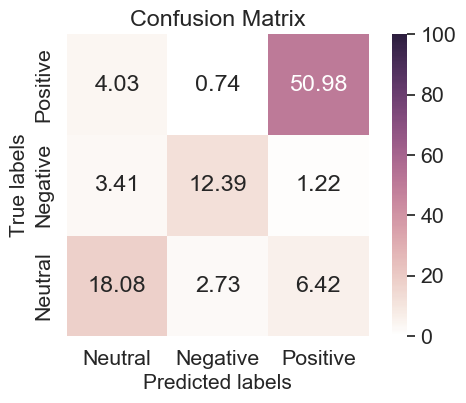
\includegraphics[width=1\columnwidth]{../img/confusion_matrix}
\protect\caption{Normalized confusion matrix}
\label{pic:conf1}
\end{figure}

\subsection{Results and Discussion}
%I tried another approach:
%Because the facebook dataset is balanced, I pretrained the model first on facebook and after reaching a decent accuracy, i further trained the model on the join data:
%for ten epochs with learning rate 5e-5 and an effecctive batch size 48.
%[[ 6240 914 2783]
%[ 1236 4447 529]
%[ 1050 273 19020]]
%Test accuracy: 0.814068837005371
%F1 metrics: 0.8087903170140932

%The pretraining model was obtained as:
%without freezing, batch size 48, 2:5e-5,4:2e-5



%Than I trained for 3 more epochs:
%[[ 6599 995 2343]
%[ 1246 4520 446]
%[ 1470 269 18604]]
%Test accuracy: 0.8145072892688808
%F1 metrics: 0.8119431050948791
%TODO  \ref{pic:conf1}

Baseline for this task is tf-idf method %TODO nekde je popsana v prni kapitole
, which resulted in 
[[ 4310   102  3015]
 [  685  1016   779]
 [  842    48 20227]]
              precision    recall  f1-score   support

           0       0.74      0.58      0.65      7427
           1       0.87      0.41      0.56      2480
           2       0.84      0.96      0.90     21117

    accuracy                           0.82     31024
   macro avg       0.82      0.65      0.70     31024
weighted avg       0.82      0.82      0.81     31024


% Please add the following required packages to your document preamble:
% \usepackage{multirow}
\begin{table}[]
\resizebox*{!}{\textheight}{\begin{tabular}{|l|l|l|l||ll|}
\hline
\multicolumn{2}{|l|}{MODEL}       & EXPE                      & LRTYPE                & Acc    & F1   \\ \hline  \hline
1  & \multirow{6}{*}{mBERT}     & czech                     & \multirow{3}{*}{Isrd} & 0,81   & 0,81 \\ \cline{1-1} \cline{3-3} \cline{5-6} 
2  &                            & zero                      &                       & 0,50   & 0,45 \\ \cline{1-1} \cline{3-3} \cline{5-6} 
3  &                            & eng                       &                       & 0,81   & 0,81 \\ \cline{1-1} \cline{3-6} 
4  &                            & czech                     & \multirow{3}{*}{cos}  & 0,83   & 0,82 \\ \cline{1-1} \cline{3-3} \cline{5-6} 
5  &                            & zero                      &                       & 0,53   & 0,48 \\ \cline{1-1} \cline{3-3} \cline{5-6} 
6  &                            & eng                       &                       & 0,83   & 0,82 \\ \hline
13 & \multirow{4}{*}{RoBECzech} & czech                     & \multirow{2}{*}{isrd} & 0,81   & 0,81 \\ \cline{1-1} \cline{3-3} \cline{5-6} 
14 &                            & zero                      &                       & 0,55   & 0,48 \\ \cline{1-1} \cline{3-6} 
16 &                            & czech                     & \multirow{2}{*}{cos}  & 0,84   & 0,84 \\ \cline{1-1} \cline{3-3} \cline{5-6} 
17 &                            & zero                      &                       & 0,58   & 0,49 \\ \hline
19 & \multirow{6}{*}{mBERT}     & czech                     & \multirow{3}{*}{Isrd} & 0,82   & 0,81 \\ \cline{1-1} \cline{3-3} \cline{5-6} 
20 &                            & zero                      &                       & 0,54   & 0,48 \\ \cline{1-1} \cline{3-3} \cline{5-6} 
21 &                            & eng                       &                       & 0,82   & 0,81 \\ \cline{1-1} \cline{3-6} 
22 &                            & czech                     & \multirow{3}{*}{cos}  & 0,83   & 0,82 \\ \cline{1-1} \cline{3-3} \cline{5-6} 
23 &                            & zero                      &                       & 0,52   & 0,47 \\ \cline{1-1} \cline{3-3} \cline{5-6} 
24 &                            & eng                       &                       & 0,83   & 0,82 \\ \hline
31 & \multirow{4}{*}{RoBECzech} & czech                     & \multirow{2}{*}{isrd} & 0,83   & 0,83 \\ \cline{1-1} \cline{3-3} \cline{5-6} 
32 &                            & zero                      &                       & 0,58   & 0,50 \\ \cline{1-1} \cline{3-6} 
34 &                            & czech                     & \multirow{2}{*}{cos}  & 0,84   & 0,84 \\ \cline{1-1} \cline{3-3} \cline{5-6} 
35 &                            & zero                      &                       & 0,58   & 0,51 \\ \hline
37 & \multirow{2}{*}{mBERT}     & \multirow{7}{*}{facebook} & Isrd                  & 0,75   & 0,75 \\ \cline{1-1} \cline{4-6} 
38 &                            &                           & cos                   & 0,76   & 0,76 \\ \cline{1-2} \cline{4-6} 
41 & \multirow{5}{*}{RoBECzech} &                           & isrd                  & 0,80   & 0,80 \\ \cline{1-1} \cline{4-6} 
42 &                            &                           & simple                & 0,79   & 0,79 \\ \cline{1-1} \cline{4-6} 
43 &                            &                           & \multirow{3}{*}{cos}  & 0,82   & 0,81 \\ \cline{1-1} \cline{5-6} 
44 &                            &                           &                       & 0,81   & 0,81 \\ \cline{1-1} \cline{5-6} 
45 &                            &                           &                       & 0,82 & 0,82 \\ \hline
46 & \multirow{2}{*}{mBERT}     & \multirow{4}{*}{facebook} & Isrd                  & 0,76   & 0,76 \\ \cline{1-1} \cline{4-6} 
47 &                            &                           & cos                   & 0,77   & 0,77 \\ \cline{1-2} \cline{4-6} 
50 & \multirow{2}{*}{RoBECzech} &                           & isrd                  & 0,80   & 0,79 \\ \cline{1-1} \cline{4-6} 
51 &                            &                           & cos                   & 0,806  & 0,80 \\ \hline
52 & \multirow{2}{*}{mBERT}     & \multirow{8}{*}{mall}     & Isrd                  & 0,83   & 0,83 \\ \cline{1-1} \cline{4-6} 
53 &                            &                           & cos                   & 0,84   & 0,84 \\ \cline{1-2} \cline{4-6} 
56 & \multirow{2}{*}{RoBECzech} &                           & isrd                  & 0,83   & 0,83 \\ \cline{1-1} \cline{4-6} 
57 &                            &                           & cos                   & 0,85   & 0,84 \\ \cline{1-2} \cline{4-6} 
58 & \multirow{2}{*}{mBERT}     &                           & Isrd                  & 0,83   & 0,83 \\ \cline{1-1} \cline{4-6} 
59 &                            &                           & cos                   & 0,84   & 0,84 \\ \cline{1-2} \cline{4-6} 
62 & \multirow{2}{*}{RoBECzech} &                           & isrd                  & 0,84   & 0,84 \\ \cline{1-1} \cline{4-6} 
63 &                            &                           & cos                   & 0,85   & 0,84 \\ \hline
64 & \multirow{2}{*}{mBERT}     & \multirow{8}{*}{csfd}     & Isrd                  & 0,81   & 0,81 \\ \cline{1-1} \cline{4-6} 
65 &                            &                           & cos                   & 0,82   & 0,82 \\ \cline{1-2} \cline{4-6} 
68 & \multirow{2}{*}{RoBECzech} &                           & isrd                  & 0,83   & 0,83 \\ \cline{1-1} \cline{4-6} 
69 &                            &                           & cos                   & 0,85   & 0,85 \\ \cline{1-2} \cline{4-6} 
70 & \multirow{2}{*}{mBERT}     &                           & Isrd                  & 0,82   & 0,82 \\ \cline{1-1} \cline{4-6} 
71 &                            &                           & cos                   & 0,82   & 0,82 \\ \cline{1-2} \cline{4-6} 
74 & \multirow{2}{*}{RoBECzech} &                           & isrd                  & 0,83   & 0,83 \\ \cline{1-1} \cline{4-6} 
75 &                            &                           & cos                   & 0,84   & 0,84 \\ \hline
\end{tabular}}
\end{table}



%Because BERT model was trained on multilingual data, it is naturally not so good in language minoritly presented in the Bert's training data. When transfering the learned knowledge to czech sentiment task, we actually want to improve model in two ways: teach it something more specific about given task, i.e., sentiment, and improve its knowledge about selected language (czech in this case). By using czech sentiment dataset, both thing are incorporated into training. To obtained better results and following the \citep{Putra}, I also selected english sentiment dataset. The idea behind is that BERT is quite good in english and maybe can learn faster useful knowledge about the given task from data in more familiar language.















